%
\documentclass[12pt,a4paper]{article}


% formatting
\usepackage[left=4cm, right=3cm, top=3cm, bottom=3cm]{geometry}

% package for nonstandard letters (umlauts etc)

\usepackage[utf8]{inputenc} 
\usepackage[]{blindtext}

%% Mathematics
\usepackage{amsmath,amsfonts,amssymb}

%% Graphics
\usepackage{graphicx}

\graphicspath{./DTfF_group_project/src/output/}

%% For nice tables
\usepackage{booktabs}

%% Line spacing
\renewcommand{\baselinestretch}{1.5}

%% Bibliography
\usepackage[
    backend=biber,
    style=bwl-FU,
    url=false,
    doi=false,
    eprint=false
]{biblatex}
\addbibresource{PMI.bib}


%% to avoid messy linebreaks
\sloppy


\begin{document}

\thispagestyle{empty}
\ \vspace{1.0cm}
\begin{center}
{\LARGE
Digital Tools for Finance: \\[0.1cm]
A fancy LATEX template for group projects\\[0.1cm]
or for a future masterthesis \\[1cm]
}

{
{\bf Project} \\
for the course \\[0.5cm]
{\bf Digital Tools for Finance } \\
{\bf at the University of Zurich} \\[0.5cm]
by\\
Igor Pozdeev and Dimitry Borisenko\\
to obtain 'Master of Try\&Error in DTfF'' \\[2.5cm]
}


\hspace{1cm}\begin{minipage}[h]{12cm}
\begin{tabbing}
Authors: \hspace{1cm} \= Patrick Storz 16-108-011 \\
\> Hubert Mrugala 19-764-265 \\
\> Kevin Steijn 19-770-429 \\
Field of Study: \> Banking and Finance \\
Subm. Date: \> 14.12.2020 \\
\end{tabbing}
\end{minipage}
\end{center}
\newpage


\begin{abstract}
Flash Eurozone PMIs for September and their signal with respect to the business cycle.
Purchasing Managers Index (PMI) is a survey that measures firms' business activity.
The surveys ask respondents (managers) to report the change in each variable (like output or employment) compared to the prior month, noting whether each has risen/improved, fallen/deteriorated or remained unchanged.Flash reading is an advanced estimate of the final PMI number based on ~85\% of total responses. It's publised about a week earlier
If PMI is 50 then nothing changed with respect to the last month. More than 50 - increased business activity. Less than 50 - decreased activity.
In addition,PMIs can be used to forecast GDP.

\end{abstract}
\newpage



\tableofcontents
\newpage


\section{Introduction}

\blindtext

\newpage




\section{Chapter}

\blindtext

\subsection{Chapter Table}

Table:
\begin{table}[ht]
\centering
\caption{Monte-Carlo-Simulation}
\label{mc-param}
\begin{tabular}{lccccc}\toprule
 &  \multicolumn{2}{c}{Exponential CEF} & & \multicolumn{2}{c}{Quadric CEF} \\
Gruppe  & $\beta_1$ & $\beta_0$ &  & $\beta_1$ & $\beta_0$ \\ \cmidrule{2-3} \cmidrule{5-6}
$c$      & 5    & 5     & & 23  & 23 \\
$x_1$   & 0.3   & 0.36  & & 3.5 & 4.55 \\
$x_2$   & 0.2   & 0.24  & & 3.5 & 4.55 \\ \bottomrule
\multicolumn{6}{p{9cm}}{\footnotesize\textit{Note}: $c$ is a constant,  $x_1$ is continuously distributed as
$N(0,1)$ and $x_2$ is a binary dummy variable with $P(x_2=1)=0.5$. }
\end{tabular}
\end{table}

\newpage
\subsection{Chapter Graphics}

 \begin{figure}[h!]
\caption{Euro Area PMI}
\centering
\label{figure1}
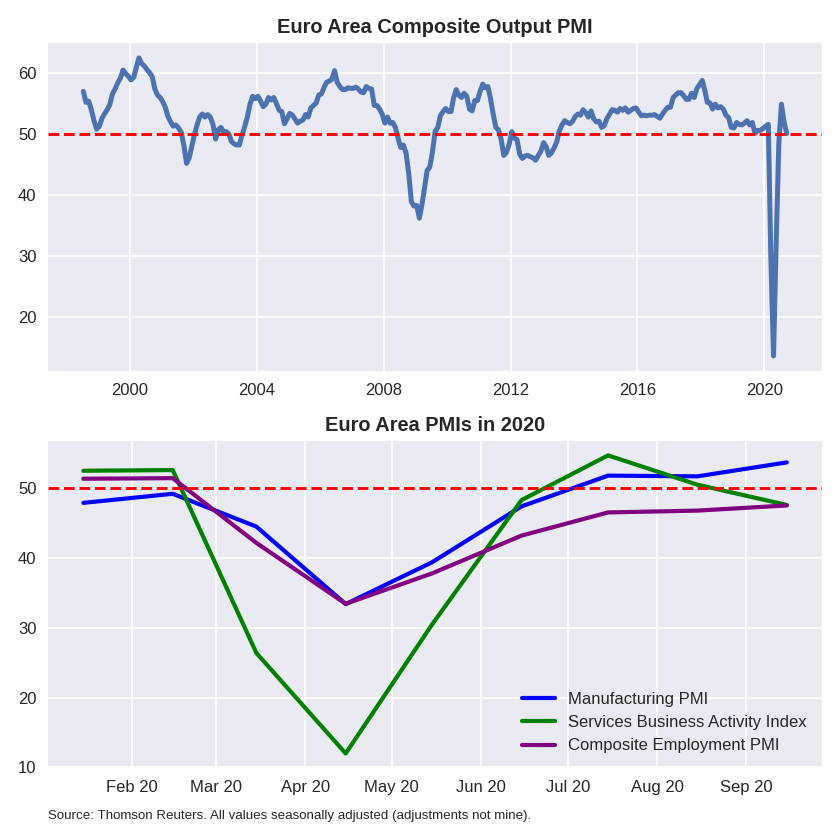
\includegraphics[width=13cm]{plots.png}
{\it Source: Thomson Reuters}
\end{figure}

\newpage 

 \begin{figure}[h!]
\caption{Europe GDP}
\centering
\label{figure1}
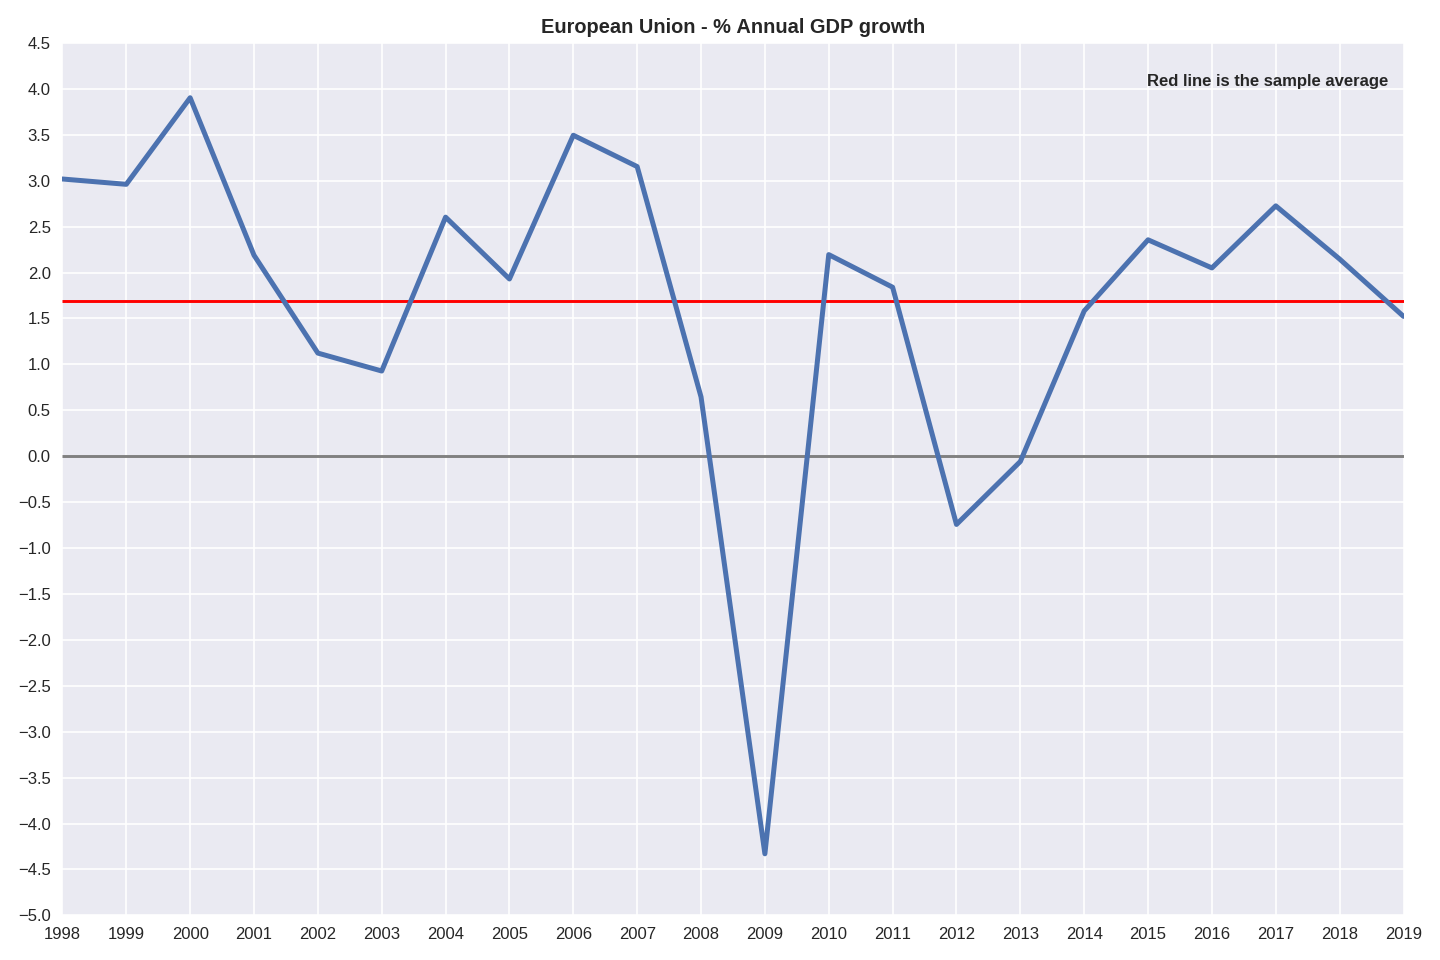
\includegraphics[width=13cm]{EU_GDP.png}
{\it Source: Worldbank}
\end{figure}

\newpage 

\begin{figure}[h!]
\caption{STOXX50E}
\centering
\label{figure1}
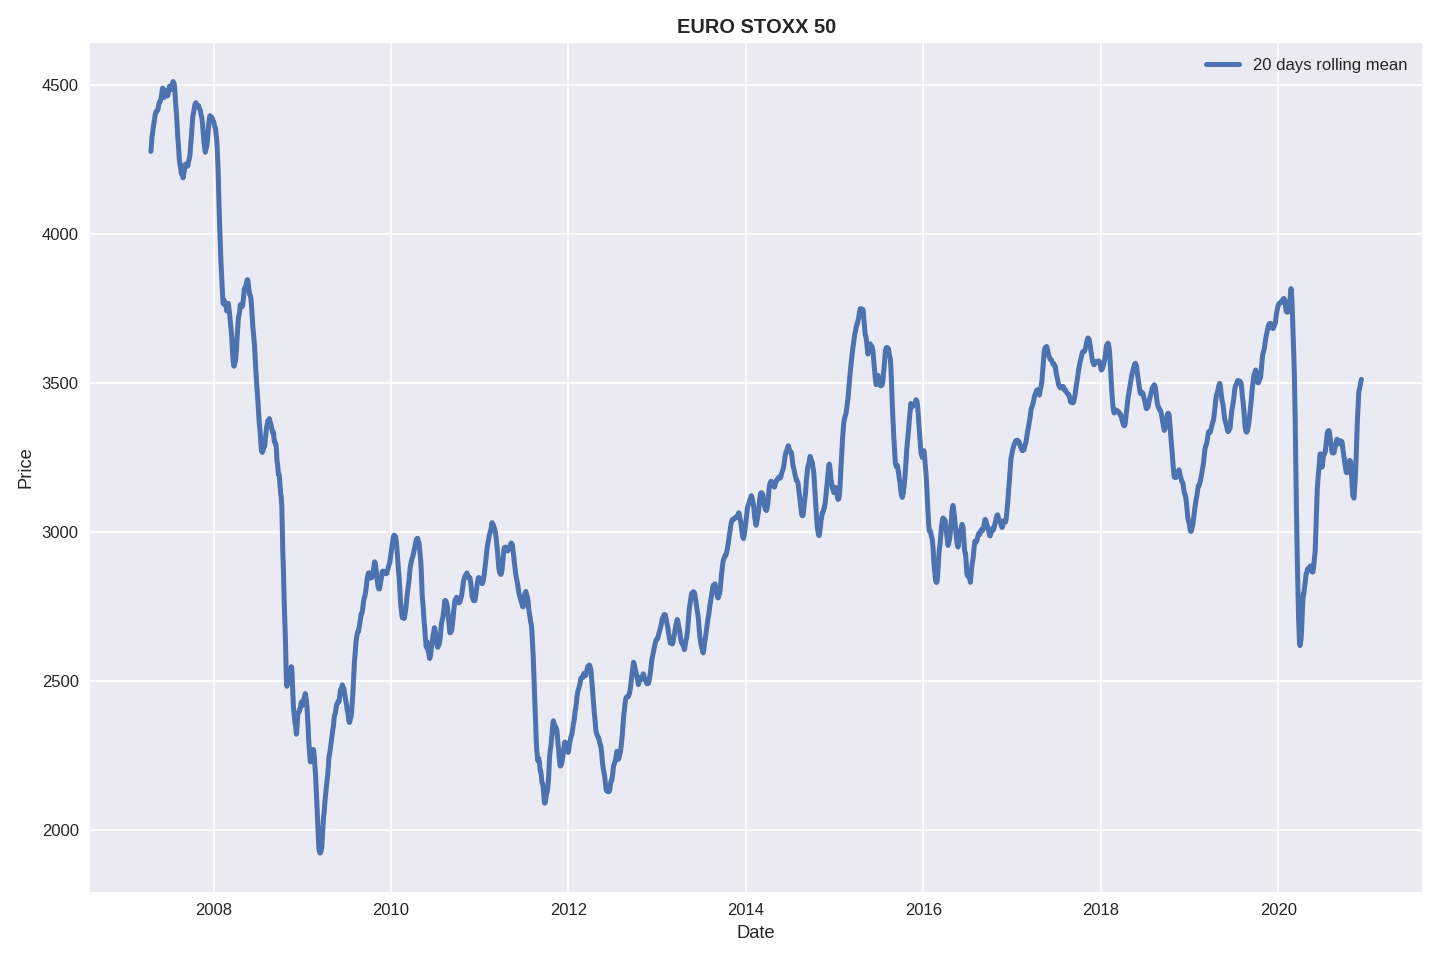
\includegraphics[width=13cm]{STOXX50E.png}
{\it Source: Yahoo}
\end{figure}

\subsection{Chapter Citation}

The working paper \cite{Koenig2002} says using the purchasing managers’ index to assess the economy’s strength and the likely direction of monetary policy.
The published paper \cite{Harris1991} mentioned something about tracking the economy.
The paper \cite{Afshar2007} shows correlations between stock return, consumer confidence, purchasing managers index and economic fluctuations. 
However,\cite{Pelaez2003} aruges that there is a better option than the PMI. 


 \subsection{Chapter Formulas}
 
Formulas 

\begin{equation}
y_i = x_i'\beta + u_i
\end{equation}

\begin{equation}
PMI =(P_{1}*1)+(P_{2}*0.5)
\end{equation}

\section{Conlusion}

\blindtext

\newpage

\section{Bibliography}

\printbibliography

\begin{description}
\item
\end{description}

\vspace{0.8cm}

\newpage
\appendix
\section{Appendix }

Additional material...

\newpage

\thispagestyle{empty}

\ \vspace{1cm}

{\bf \huge Declaration of independence} \\[0.4cm]

I hereby declare that I am writing this paper independently and that I do not
other than the given sources. I have marked as such all passages that were taken literally or analogously from sources. I am aware that otherwise the Senate, in accordance with Article 36 paragraph 1 letter o of the Law of 5 September 1996 on the University, will withdraw the title conferred on the basis of this work
is authorized.\\[0.5cm]

Zürich, DD.MM.YYYY \hspace{5cm} \hrulefill \hspace{1cm} \\[0cm]
\begin{minipage}[h]{15cm} \hspace{10.5cm}  {\small (Unterschrift)}
\end{minipage}



\end{document}
